\chapter{Solides et volumes}\label{ch:g9:solids}

La géométrie de l'espace commence par une petite famille de \omterm{def:g5:solids:def}{solides} ---
\omterm{def:g7:areas:prism}{prismes}, \omterm{def:g7:areas:prism}{cylindres}, \omterm{def:g8:solids:def}{pyramides}, \omterm{def:g8:solids:def}{cônes}, sphères --- et deux questions~:
combien contiennent-ils (\omterm{def:g6:measure:volume}{volume}), et que voit-on lorsqu'on les coupe
(\omterm{prop:g9:solids:sections}{sections})~? Le chapitre se clôt sur un fait d'une grande importance
pratique~: homothétier un \omterm{def:g5:solids:def}{solide} par $k$ multiplie son \omterm{def:g6:measure:volume}{volume} par $k^3$.

\section{Les solides classiques et leurs volumes}

\begin{theorem}[Formules de volume]\label{thm:g9:solids:volumes}
Noter $B$ l'\omterm{def:g6:measure:area}{aire} de la base et $h$ la hauteur (la distance entre la base
et la \omterm{def:g5:solids:def}{face} ou le \omterm{def:g5:solids:def}{sommet} opposé).
\begin{center}
\renewcommand{\arraystretch}{1.5}
\begin{tabular}{l|l}
\omterm{def:g5:solids:def}{solide} & \omterm{def:g6:measure:volume}{volume} \\
\hline
\omterm{def:g7:areas:prism}{prisme}, \omterm{def:g7:areas:prism}{cylindre} & $V = B \times h$ \\[5pt]
\omterm{def:g8:solids:def}{pyramide}, \omterm{def:g8:solids:def}{cône} & $V = \dfrac13\, B \times h$ \\[5pt]
sphère de \omterm{def:g3:shapes:shapes}{rayon} $r$ & $V = \dfrac43\,\pi r^3$ \\
\end{tabular}
\end{center}
Pour un \omterm{def:g7:areas:prism}{cylindre} et un \omterm{def:g8:solids:def}{cône} de \omterm{def:g3:shapes:shapes}{rayon} $r$, l'\omterm{def:g6:measure:area}{aire} de base est
$B = \pi r^2$~; l'\omterm{def:g6:measure:area}{aire} de surface de la sphère est $4\pi r^2$.
\end{theorem}
\admitted

\begin{omfigure}
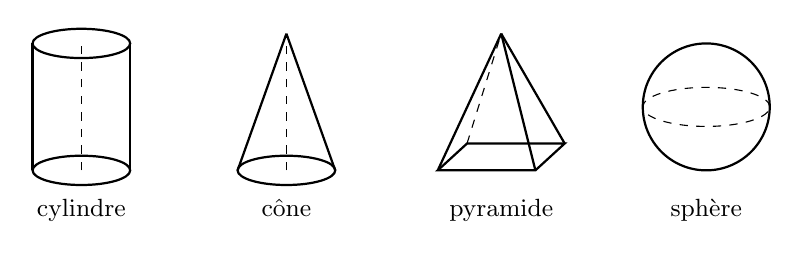
\begin{tikzpicture}[scale=0.62]
  % cylinder
  \draw[thick] (0,0) ellipse (1 and 0.3);
  \draw[thick] (-1,0) -- (-1,2.6);
  \draw[thick] (1,0) -- (1,2.6);
  \draw[thick] (0,2.6) ellipse (1 and 0.3);
  \draw[dashed] (0,0) -- (0,2.6);
  \node[below, font=\small] at (0,-0.4) {cylindre};
  % cone
  \begin{scope}[xshift=4.2cm]
  \draw[thick] (0,0) ellipse (1 and 0.3);
  \draw[thick] (-1,0) -- (0,2.8);
  \draw[thick] (1,0) -- (0,2.8);
  \draw[dashed] (0,0) -- (0,2.8);
  \node[below, font=\small] at (0,-0.4) {cône};
  \end{scope}
  % pyramid
  \begin{scope}[xshift=8.4cm]
  \draw[thick] (-1.1,0) -- (0.9,0) -- (1.5,0.55) -- (-0.5,0.55) -- cycle;
  \draw[thick] (-1.1,0) -- (0.2,2.8);
  \draw[thick] (0.9,0) -- (0.2,2.8);
  \draw[thick] (1.5,0.55) -- (0.2,2.8);
  \draw[dashed] (-0.5,0.55) -- (0.2,2.8);
  \node[below, font=\small] at (0.2,-0.4) {pyramide};
  \end{scope}
  % sphere
  \begin{scope}[xshift=12.8cm]
  \draw[thick] (0,1.3) circle (1.3);
  \draw[dashed] (0,1.3) ellipse (1.3 and 0.4);
  \node[below, font=\small] at (0,-0.4) {sphère};
  \end{scope}
\end{tikzpicture}

{\small Les \omterm{def:g5:solids:def}{solides} de ce chapitre. Pour chacun, le \omterm{def:g6:measure:volume}{volume} fait
intervenir une \omterm{def:g6:measure:area}{aire} de base et une hauteur --- sauf la sphère, qui n'a
besoin que de son \omterm{def:g3:shapes:shapes}{rayon}.}
\end{omfigure}

\begin{example}\label{ex:g9:solids:volumes}
Une boîte de conserve cylindrique a pour \omterm{def:g3:shapes:shapes}{rayon} $4$ cm et pour hauteur
$10$ cm~:
\[
V = \pi r^2 h = \pi \times 16 \times 10 = 160\pi \approx 503 \text{ cm}^3
\approx 0.5 \text{ L}.
\]
Un \omterm{def:g8:solids:def}{cône} de même base et même hauteur contient le tiers de cela~:
$\frac{160\pi}{3} \approx 168$ cm$^3$. Une sphère de \omterm{def:g3:shapes:shapes}{rayon} $4$ cm~:
$V = \frac43 \pi \times 64 = \frac{256\pi}{3} \approx 268$ cm$^3$.
\end{example}

\begin{example}[Une pyramide étape par étape]\label{ex:g9:solids:pyramid}
Une \omterm{def:g8:solids:def}{pyramide} a une base carrée de côté $6$ m et une hauteur de $5$ m.
\begin{enumerate}
  \item \omterm{def:g6:measure:area}{Aire} de base~: $B = 6^2 = 36$ m$^2$.
  \item \omterm{def:g6:measure:volume}{Volume}~: $V = \frac13 \times 36 \times 5 = 60$ m$^3$.
\end{enumerate}
Attention aux unités~: si le côté était donné en cm et la hauteur en m,
il faudrait convertir l'un d'eux d'abord.
\end{example}

\section{Sections par des plans}

\begin{proposition}[Sections des solides classiques]\label{prop:g9:solids:sections}
Couper un \omterm{def:g5:solids:def}{solide} par un plan \omterm{def:g2:mult:def}{produit} une figure plane, sa
\emph{section}\index{section}~:
\begin{itemize}
  \item un \omterm{def:g7:areas:prism}{prisme} ou un \omterm{def:g7:areas:prism}{cylindre} coupé \emph{parallèlement à sa base}
        donne une copie de la base, à toute hauteur~;
  \item une \omterm{def:g8:solids:def}{pyramide} ou un \omterm{def:g8:solids:def}{cône} coupé parallèlement à sa base donne une
        \emph{réduction} de la base~: à distance $d$ du \omterm{def:g5:solids:def}{sommet}, le
        \omterm{def:g9:thales:scaling}{facteur d'échelle} est $k = \frac{d}{h}$~;
  \item une sphère de \omterm{def:g3:shapes:shapes}{rayon} $r$ coupée par un plan à distance $d < r$
        du centre donne un cercle de \omterm{def:g3:shapes:shapes}{rayon} $\sqrt{r^2 - d^2}$ (par le
        théorème de Pythagore).
\end{itemize}
\end{proposition}
\admitted

\begin{omfigure}
\begin{tikzpicture}[scale=0.75]
  % cone with section
  \draw[thick] (0,0) ellipse (1.5 and 0.45);
  \draw[thick] (-1.5,0) -- (0,4.0);
  \draw[thick] (1.5,0) -- (0,4.0);
  \draw[omThm, thick, fill=omThm!12] (0,2.4) ellipse (0.6 and 0.18);
  \draw[dashed] (0,0) -- (0,4.0);
  \node[right, font=\small] at (0.1,4.0) {sommet};
  \draw[Stealth-Stealth, thin] (2.1,0) -- (2.1,4.0);
  \node[right, font=\small] at (2.1,2.0) {$h$};
  \draw[Stealth-Stealth, thin, omThm] (0.9,2.4) -- (0.9,4.0);
  \node[right, font=\small, omThm] at (0.92,3.2) {$d$};
  % sphere with section
  \begin{scope}[xshift=7.6cm]
  \draw[thick] (0,2) circle (1.8);
  \draw[omThm, thick, fill=omThm!12] (0,2.9) ellipse (1.56 and 0.4);
  \fill (0,2) circle (1.5pt) node[below, font=\small] {$O$};
  \draw[thin] (0,2) -- (0,2.9) node[midway, left, font=\small] {$d$};
  \draw[thin] (0,2.9) -- (1.56,2.9)
    node[midway, above, font=\small] {$\sqrt{r^2 - d^2}$};
  \draw[thin] (0,2) -- (-1.27,0.72)
    node[midway, below right=-3pt, font=\small] {$r$};
  \end{scope}
\end{tikzpicture}

{\small Gauche~: couper un \omterm{def:g8:solids:def}{cône} parallèlement à sa base à distance $d$
du \omterm{def:g5:solids:def}{sommet} donne un disque réduit par $k = \frac dh$. Droite~: un plan à
distance $d$ du centre d'une sphère la coupe en un cercle de \omterm{def:g3:shapes:shapes}{rayon}
$\sqrt{r^2 - d^2}$.}
\end{omfigure}

\begin{example}\label{ex:g9:solids:section}
Un \omterm{def:g8:solids:def}{cône} a pour \omterm{def:g3:shapes:shapes}{rayon} de base $6$ et pour hauteur $9$. La \omterm{prop:g9:solids:sections}{section} par un
plan \omterm{def:g6:lines:perp}{parallèle} à la base, à distance $3$ du \omterm{def:g5:solids:def}{sommet}, est un disque réduit
par $k = \frac39 = \frac13$~: son \omterm{def:g3:shapes:shapes}{rayon} est $6 \times \frac13 = 2$.

Une sphère de \omterm{def:g3:shapes:shapes}{rayon} $5$ est coupée par un plan à distance $3$ de son
centre~: la \omterm{prop:g9:solids:sections}{section} est un cercle de \omterm{def:g3:shapes:shapes}{rayon} $\sqrt{25 - 9} = 4$.
\end{example}

\section{Homothétie des solides}

\begin{theorem}[Effet d'une homothétie sur longueurs, aires, volumes]\label{thm:g9:solids:scaling}
Lorsqu'un \omterm{def:g5:solids:def}{solide} est agrandi ou réduit par le \omterm{def:g9:thales:scaling}{facteur d'échelle}
$k > 0$~:
\begin{itemize}
  \item toutes les longueurs sont multipliées par $k$~;
  \item toutes les \omterm{def:g6:measure:area}{aires} sont multipliées par $k^2$~;
  \item tous les \omterm{def:g6:measure:volume}{volumes} sont multipliés par $k^3$.
\end{itemize}
\end{theorem}
\admitted

\begin{example}\label{ex:g9:solids:scaling}
Une voiture miniature à l'échelle $\frac{1}{18}$~: les longueurs sont
celles de la voiture réelle multipliées par $k = \frac{1}{18}$, la
surface peinte multipliée par $k^2 = \frac{1}{324}$, et le \omterm{def:g6:measure:volume}{volume} par
$k^3 = \frac{1}{5832}$.

Doubler le \omterm{def:g3:shapes:shapes}{rayon} d'une sphère ($k = 2$) multiplie son \omterm{def:g6:measure:volume}{volume} par
$2^3 = 8$~: vérifier sur la formule,
$\frac43\pi (2r)^3 = \frac43 \pi \times 8r^3$.
\end{example}

\begin{example}[Tronc de cône]\label{ex:g9:solids:truncated}
Un \omterm{def:g8:solids:def}{cône} de hauteur $9$ et de \omterm{def:g3:shapes:shapes}{rayon} de base $6$ (\omterm{def:g6:measure:volume}{volume}
$\frac13 \pi \times 36 \times 9 = 108\pi$) est coupé à distance $3$ du
\omterm{def:g5:solids:def}{sommet}, et le petit \omterm{def:g8:solids:def}{cône} au-dessus de la coupe est enlevé. Le petit \omterm{def:g8:solids:def}{cône}
est la réduction par $k = \frac13$, donc son \omterm{def:g6:measure:volume}{volume} est
$108\pi \times \left(\frac13\right)^3 = 4\pi$. Le \omterm{def:g5:solids:def}{solide} restant (un
\emph{tronc de \omterm{def:g8:solids:def}{cône}}) a pour \omterm{def:g6:measure:volume}{volume} $108\pi - 4\pi = 104\pi \approx 327$.
\end{example}

\section{Exercices}

\begin{exercise}[$\star$]\label{exo:g9:solids:1}
Calculer les \omterm{def:g6:measure:volume}{volumes}~: un \omterm{def:g5:solids:def}{pavé} (\omterm{def:g7:areas:prism}{prisme} rectangulaire) de dimensions
$4 \times 5 \times 12$~; un \omterm{def:g7:areas:prism}{cylindre} de \omterm{def:g3:shapes:shapes}{rayon} $3$ et de hauteur $7$
(valeur exacte avec $\pi$, puis arrondie à l'unité).
\end{exercise}

\begin{exercise}[$\star$]\label{exo:g9:solids:2}
Calculer le \omterm{def:g6:measure:volume}{volume} d'un \omterm{def:g8:solids:def}{cône} de \omterm{def:g3:shapes:shapes}{rayon} $5$ et de hauteur $12$, et d'une
\omterm{def:g8:solids:def}{pyramide} de base rectangulaire $8 \times 3$ et de hauteur $10$.
\end{exercise}

\begin{exercise}[$\star$]\label{exo:g9:solids:3}
Calculer le \omterm{def:g6:measure:volume}{volume} et l'\omterm{def:g6:measure:area}{aire} de surface d'une sphère de \omterm{def:g3:shapes:shapes}{rayon} $6$
(valeurs exactes avec $\pi$).
\end{exercise}

\begin{exercise}[$\star$]\label{exo:g9:solids:4}
Une sphère de \omterm{def:g3:shapes:shapes}{rayon} $10$ est coupée par un plan à distance $8$ de son
centre. Quel est le \omterm{def:g3:shapes:shapes}{rayon} du cercle de \omterm{prop:g9:solids:sections}{section}~?
\end{exercise}

\begin{exercise}[$\star\star$]\label{exo:g9:solids:5}
Un \omterm{def:g8:solids:def}{cône} a pour \omterm{def:g3:shapes:shapes}{rayon} de base $8$ et pour hauteur $12$. Un plan \omterm{def:g6:lines:perp}{parallèle}
à la base le coupe à distance $9$ du \omterm{def:g5:solids:def}{sommet}. Calculer le \omterm{def:g3:shapes:shapes}{rayon} de la
\omterm{prop:g9:solids:sections}{section}, puis le \omterm{def:g6:measure:volume}{volume} du petit \omterm{def:g8:solids:def}{cône} au-dessus de la coupe.
\end{exercise}

\begin{exercise}[$\star\star$]\label{exo:g9:solids:6}
Un verre cylindrique de \omterm{def:g3:shapes:shapes}{rayon} intérieur $3$ cm contient de l'eau jusqu'à
une hauteur de $10$ cm. Une bille de \omterm{def:g3:shapes:shapes}{rayon} $2$ cm y est entièrement
immergée. De combien le niveau d'eau monte-t-il~? (Le \omterm{def:g6:measure:volume}{volume} ajouté se
répartit sur l'\omterm{def:g6:measure:area}{aire} de base du verre~; donner la montée exacte, puis
\omterm{def:g4:numbers:round}{arrondir} au millimètre.)
\end{exercise}

\begin{exercise}[$\star\star$]\label{exo:g9:solids:7}
Une recette remplit un moule sphérique de \omterm{def:g3:shapes:shapes}{rayon} $6$ cm. On ne dispose que
d'un moule sphérique de \omterm{def:g3:shapes:shapes}{rayon} $3$ cm. Combien de petits moules peut-on
remplir~? (Répondre sans calculer explicitement ni l'un ni l'autre
\omterm{def:g6:measure:volume}{volume}.)
\end{exercise}

\begin{exercise}[$\star\star$]\label{exo:g9:solids:8}
La Grande \omterm{def:g8:solids:def}{Pyramide} de Gizeh a une base carrée de côté environ $230$ m et
une hauteur d'environ $147$ m. Estimer son \omterm{def:g6:measure:volume}{volume}, et l'exprimer en
millions de mètres cubes.
\end{exercise}

\begin{exercise}[$\star\star\star$]\label{exo:g9:solids:9}
Un entonnoir en forme de \omterm{def:g8:solids:def}{cône} de \omterm{def:g3:shapes:shapes}{rayon} $6$ cm et de hauteur $12$ cm,
\omterm{def:g5:solids:def}{sommet} en bas, est rempli d'eau jusqu'à la \omterm{def:g3:division:half}{moitié} de sa \emph{hauteur}
(mesurée depuis le \omterm{def:g5:solids:def}{sommet}).
\begin{enumerate}
  \item Quelle \omterm{def:g9:fractions:fraction}{fraction} du \omterm{def:g6:measure:volume}{volume} de l'entonnoir est remplie~?
  \item Si au contraire on le remplit de la \omterm{def:g3:division:half}{moitié} de son \emph{\omterm{def:g6:measure:volume}{volume}}
        d'eau, montrer que la hauteur d'eau $d$ satisfait
        $\left(\frac{d}{12}\right)^3 = \frac12$, et donner $d$ au
        millimètre près ($\sqrt[3]{0.5} \approx 0.7937$).
\end{enumerate}
\end{exercise}

\section{Problème~: la pierre tombale d'Archimède}

\begin{problem}[{Devoir maison --- la sphère vaut les deux tiers de
son cylindre (deux fois plutôt qu'une), l'empilement 1:2:3, et la loi
du carré-cube qui interdit les géants}]
\label{pb:g9:solids:1}
Archimède a démontré bien des théorèmes, mais l'un d'eux le rendit si
fier qu'il demanda que sa \emph{figure} fût gravée sur son tombeau~:
une sphère nichée dans son \omterm{def:g7:areas:prism}{cylindre} le plus juste. Un siècle plus
tard, l'écrivain romain Cicéron, fouillant les ronces près de
Syracuse, reconnut la tombe «~à la sphère et au \omterm{def:g7:areas:prism}{cylindre}~». Ce
problème retrouve ce que la gravure encode --- un double miracle des
deux tiers --- puis suit \omterm{def:g6:measure:volume}{volumes} et surfaces
(\cref{thm:g9:solids:volumes}, \cref{thm:g9:solids:scaling}) jusqu'à
une loi qui gouverne les géants, les fourmis et le refroidissement
des planètes.

\medskip
\noindent\textbf{Partie I --- La gravure décodée.}
Une sphère de \omterm{def:g3:shapes:shapes}{rayon} $r$ tient exactement dans un \omterm{def:g7:areas:prism}{cylindre}~: même
\omterm{def:g3:shapes:shapes}{rayon}, hauteur $2r$.
\begin{enumerate}
  \item Calculer le \omterm{def:g6:measure:volume}{volume} du \omterm{def:g7:areas:prism}{cylindre} en fonction de $r$.
  \item Calculer le rapport du \omterm{def:g6:measure:volume}{volume} de la sphère à celui du
        \omterm{def:g7:areas:prism}{cylindre}. Pourquoi Archimède a-t-il pu se réjouir que la
        réponse ne contienne ni $\pi$ ni $r$~?
  \item Passons aux surfaces~: comparer l'\omterm{def:g6:measure:area}{aire} de la sphère à
        l'\omterm{def:g6:measure:area}{aire} \emph{totale} du \omterm{def:g7:areas:prism}{cylindre} (partie latérale plus les
        deux disques). Quel rapport apparaît --- encore une fois~?
  \item L'espace vide entre la sphère et le \omterm{def:g7:areas:prism}{cylindre} a pour \omterm{def:g6:measure:volume}{volume}
        $2\pi r^3 - \frac43\pi r^3$. Montrer que ce \omterm{def:g3:division:remainder}{reste} vaut
        exactement le \omterm{def:g6:measure:volume}{volume} de \emph{deux \omterm{def:g8:solids:def}{cônes}} de \omterm{def:g3:shapes:shapes}{rayon} $r$ et de
        hauteur $r$.
  \item Un ballon de basket de \omterm{def:g3:shapes:shapes}{rayon} $12$ cm est vendu dans la boîte
        cylindrique la plus juste. Calculer les deux \omterm{def:g6:measure:volume}{volumes} (à
        $100$ cm$^3$ près) et le pourcentage de la boîte qui reste
        vide.
\end{enumerate}

\medskip
\noindent\textbf{Partie II --- Bols, moules et lunes.}
\begin{enumerate}[resume]
  \item Un bol hémisphérique a un \omterm{def:g3:shapes:shapes}{rayon} de $10$ cm. Calculer sa
        \omterm{def:g2:measure:units}{contenance}, en cm$^3$ puis en litres (au décilitre près).
  \item L'empilement 1:2:3~: un \omterm{def:g8:solids:def}{cône}, une demi-boule et un \omterm{def:g7:areas:prism}{cylindre},
        tous de \omterm{def:g3:shapes:shapes}{rayon} $10$ cm et de hauteur $10$ cm. Calculer les
        trois \omterm{def:g6:measure:volume}{volumes} et vérifier la légendaire proportion
        $1 : 2 : 3$. (Archimède aurait apprécié celle-ci aussi.)
  \item Une sphère de chocolat de \omterm{def:g3:shapes:shapes}{rayon} $3$ cm est fondue dans un
        moule cylindrique de \omterm{def:g3:shapes:shapes}{rayon} $3$ cm. Quelle hauteur le
        chocolat atteint-il~? (\omterm{def:g9:fractions:fraction}{Fraction} exacte, puis au millimètre
        près.)
  \item Le \omterm{def:g3:shapes:shapes}{rayon} de la Terre vaut environ $6\,371$ km, celui de la
        Lune environ $1\,737$ km. Calculer le rapport des \omterm{def:g3:shapes:shapes}{rayons},
        puis --- avec \cref{thm:g9:solids:scaling} --- le rapport
        des \omterm{def:g6:measure:volume}{volumes}~: combien de Lunes tiendraient dans une Terre
        creuse, en \omterm{def:g6:measure:volume}{volume}~?
  \item D'après le même théorème~: quel est le rapport
        Terre--Lune des \emph{\omterm{def:g6:measure:area}{aires}}~? Et en général, lorsque le
        \omterm{def:g3:shapes:shapes}{rayon} d'un ballon double, qu'arrive-t-il à son \omterm{def:g6:measure:volume}{volume} et à
        sa surface~? Énoncer la \emph{loi du \omterm{def:g5:solids:def}{carré-cube}}~: quand une
        forme grandit, les \omterm{def:g6:measure:volume}{volumes} distancent les surfaces.
\end{enumerate}

\medskip
\noindent\textbf{Partie III --- La loi du \omterm{def:g5:solids:def}{carré-cube} gouverne le
monde.}
\begin{enumerate}[resume]
  \item L'argument de Galilée contre les géants~: imaginer un être
        humain agrandi d'un facteur $10$, toutes proportions
        conservées. Par quel facteur son poids est-il multiplié (le
        poids suit le \omterm{def:g6:measure:volume}{volume})~? Par quel facteur la \omterm{prop:g9:solids:sections}{section} de ses
        os est-elle multipliée (c'est une \omterm{def:g6:measure:area}{aire})~? Par quel facteur,
        dès lors, la \emph{pression} sur chaque centimètre carré
        d'os est-elle multipliée --- et qu'advient-il du géant~?
  \item La même loi, à l'envers, explique les exploits des
        fourmis~: la force suit la \omterm{prop:g9:solids:sections}{section} des muscles (une \omterm{def:g6:measure:area}{aire}),
        le poids suit le \omterm{def:g6:measure:volume}{volume}. Pour un animal $100$ fois plus
        petit dans toutes les directions, par quels facteurs le
        poids et la force sont-ils divisés, et par quel facteur le
        rapport force sur poids s'améliore-t-il~?
  \item La chaleur est produite par le \omterm{def:g6:measure:volume}{volume} du corps et perdue par
        sa surface. Montrer que, pour une sphère, le rapport surface
        sur \omterm{def:g6:measure:volume}{volume} vaut $\frac{3}{r}$, et le calculer pour $r = 1$
        puis $r = 2$. Qui refroidit le plus vite, une souris ou un
        ours --- et pourquoi les bébés ont-ils besoin d'un bonnet en
        hiver~?
  \item Deux oranges sphériques, de \omterm{def:g3:shapes:shapes}{rayons} $4$ cm et $5$ cm, sont
        vendues au même prix. Calculer le rapport de leurs \omterm{def:g6:measure:volume}{volumes}~:
        combien d'orange en plus la grosse donne-t-elle pour le même
        argent~?
  \item Bouquet final~: décrire précisément ce que la figure de la
        pierre tombale encode --- les deux «~deux tiers~» des
        questions 2 et 3 --- et répondre à Cicéron en une phrase~:
        pourquoi un mathématicien choisirait-il, plutôt que toutes
        les conquêtes de son génie d'ingénieur, une sphère dans un
        \omterm{def:g7:areas:prism}{cylindre}~?
\end{enumerate}
\end{problem}
